
%\documentclass[conference]{IEEEtran}
\documentclass[10pt,conference]{IEEEtran}

\pagestyle{plain}

\usepackage[english,american]{babel}
\usepackage{graphicx}
\usepackage{subfigure}
\usepackage{amsmath}
\usepackage{multirow}
\usepackage{multicol}
\usepackage{float}
\usepackage{algorithm}
\usepackage{algorithmic}
\usepackage[colorlinks, linkcolor=red, anchorcolor=green, citecolor=blue]{hyperref}
\usepackage{cite}
\usepackage{balance}
\usepackage{color}
\usepackage[square,sort,comma,numbers]{natbib}
\usepackage{url}
\usepackage{diagbox}
\usepackage{enumerate}
\usepackage{setspace}
\let\labelindent\relax
\usepackage{enumitem}
\usepackage{indentfirst}
\usepackage{booktabs}
\usepackage{tikz}
\usepackage{listings}
\usepackage{etoolbox}
\usepackage{setspace}

\hyphenation{op-tical net-works semi-conduc-tor}
%\renewcommand{\baselinestretch}{0.985}
%\renewcommand{\captionfont}{\linespread{1.5}\normalsize}

%\renewcommand{\thesection}{\arabic{section}}
%\renewcommand{\thesubsection}{\thesection.\arabic{subsection}}
%\renewcommand{\thesubsubsection}{\thesubsection.\arabic{subsubsection}}

%\makeatletter
%\def\@seccntformat#1{\@ifundefined{#1@cntformat}%
%   {\csname the#1\endcsname\quad}%       default
%   {\csname #1@cntformat\endcsname}}%    enable individual control
%\newcommand\section@cntformat{}
%\makeatother

\renewcommand{\algorithmicrequire}{\textbf{Input:}}
\renewcommand{\algorithmicensure}{\textbf{Output:}}
%\usepackage{setspace}
%\usepackage{epsfig,graphics,subfigure,psfrag,amsmath,amssymb}
\newcommand\FIXME[1]{\textcolor{red}{FIX:}\textcolor{red}{#1}}
\newcommand\FIXED[1]{\textcolor{blue}{FIXED: }\textcolor{blue}{#1}}

%\def\@IEEEsectpunct{.\ \,}
%\def\paragraph{\@startsection{paragraph}{4}{\z@}{1.5ex plus 1.5ex minus 0.5ex}%
%{0ex}{\normalfont\normalsize\sffamily\bfseries}}


\newcommand{\circled}[2][]{\tikz[baseline=(char.base)]
    {\node[shape = circle, draw, inner sep = 1pt]
    (char) {\phantom{\ifblank{#1}{#2}{#1}}};%
    \node at (char.center) {\makebox[0pt][c]{#2}};}}
\robustify{\circled}

\begin{document}
%\setcopyright{acmcopyright}

\title{Using Facial Behavior Biometric Modalities for Smartphone Authentication}
\author{
%\IEEEauthorblockN{Guixin Ye\IEEEauthorrefmark{2},
%Zhanyong Tang$^{*,}$\IEEEauthorrefmark{2}\thanks{*Corresponding authors: Zhanyong Tang and Zheng Wang},
%Dingyi Fang\IEEEauthorrefmark{2},
%Xiaojiang Chen\IEEEauthorrefmark{2},
%Kwang In Kim\IEEEauthorrefmark{3},
%Ben Taylor\IEEEauthorrefmark{4}, and
%Zheng Wang$^{*,}$\IEEEauthorrefmark{4}}
%\IEEEauthorblockA{\IEEEauthorrefmark{2}School of Information Science and Technology, Northwest University, China\\Email:  gxye@stumail.nwu.edu.cn, \{zytang, dyf, xjchen\}@nwu.edu.cn}
%\IEEEauthorblockA{\IEEEauthorrefmark{3}Department of Computer Science, University of Bath, UK\\Email: k.kim@bath.ac.uk}
%\IEEEauthorblockA{\IEEEauthorrefmark{4}School of Computing and Communications, Lancaster University, UK\\Email: \{b.d.taylor, z.wang\}@lancaster.ac.uk}
}

\IEEEoverridecommandlockouts
\makeatletter\def\@IEEEpubidpullup{9\baselineskip}\makeatother
\IEEEpubid{\parbox{\columnwidth}{Permission to freely reproduce all or part
    of this paper for noncommercial purposes is granted provided that
    copies bear this notice and the full citation on the first
    page. Reproduction for commercial purposes is strictly prohibited
    without the prior written consent of the Internet Society, the
    first-named author (for reproduction of an entire paper only), and
    the author's employer if the paper was prepared within the scope
    of employment.  \\
    NDSS '17, 26 February -1 March 2017, San Diego, CA, USA\\
    Copyright 2017 Internet Society, ISBN 1-891562-41-X\\
    http://dx.doi.org/10.14722/ndss.2017.23xxx
}
\hspace{\columnsep}\makebox[\columnwidth]{}}

\maketitle

\begin{abstract}

%Pattern lock is widely used as a mechanism for authentication and authorization on Android devices. This paper presents a novel video-based attack to reconstruct Android lock patterns from video footage filmed using a mobile phone camera. Unlike prior attacks on pattern lock, our approach does not require the video to capture any content displayed on the screen. Instead, we employ a computer vision algorithm to track the fingertip movements to infer the pattern. Using the geometry information extracted from the tracked fingertip motions, our approach is able to accurately identify a small number of
%(often one) candidate patterns to be tested by an adversary.
%We  thoroughly evaluated our approach using 120 unique patterns collected from 215 independent users, by applying it to reconstruct patterns from video footage filmed using smartphone cameras. Experimental results show that our approach can break over 95\% of the patterns in five attempts before the device is automatically locked by the Android operating system. We discovered that, in contrast to many people's belief, complex patterns do not offer stronger protection under our attacking scenarios. This is demonstrated by the fact that we are able to break all but one complex patterns
%as opposed to  60\% of the simple patterns in the first attempt. Since our threat model is common in
%day-to-day life, this paper calls for the community to revisit the risks of using Android pattern lock to protect sensitive information.
\\
\end{abstract}


%\begin{CCSXML}
%<ccs2012>
%<concept>
%<concept_id>10002978.10002991.10002992.10011618</concept_id>
%<concept_desc>Security and privacy~Graphical / visual passwords</concept_desc>
%<concept_significance>500</concept_significance>
%</concept>
%<concept>
%<concept_id>10002978.10003014.10003017</concept_id>
%<concept_desc>Security and privacy~Mobile and wireless security</concept_desc>
%<concept_significance>300</concept_significance>
%</concept>
%</ccs2012>
%\end{CCSXML}
%
%\ccsdesc[500]{Security and privacy~Graphical / visual passwords}
%\ccsdesc[300]{Security and privacy~Mobile and wireless security}
%
%\printccsdesc
% no keywords
%\keywords{Side-channel Attack, Android Pattern Lock, Authentication, Motion Tracking, Vision Analysis}\\

%TODO:
% Read: A pilot study on the security of pattern screen-lock methods and soft side channel attacks
\section{Introduction}
Smartphone is easily lost or stolen by an attacker as its small size. This may result in privacy leakage and finance lost. It is reported by lookout.com that nearly \$2.5 billion worth of devices were lost or stolen in 2011\cite{lookout-survey}.
\section{Background}
    \subsection{Facial Expression}
        Facial expression is driven by a series of muscles movements beneath the skin of the face. These movements convey the individual's emotion status so that facial expressions are a form of nonverbal language to convey information in social interaction. Studies have discovered that there are at least 21 kinds of facial expressions including six basic expressions~\cite{Ekman1972} and compound expressions consisted of the six basic expressions~\cite{Du2014Compound}. Psychologist stated that almost 55\% volume of information are conveyed through facial expression in communication~\cite{Lebow2009Communication}. Thus, facial expressions carry a large amount of information in daily communication. Facial expression is pervasively used in human centered interfaces such as virtual reality~\cite{Bekele2013Understanding}, user profiling~\cite{Arapakis2009Integrating} and mental health~\cite{Acharya2012Impact} as it can present the individual's mental status. Unlike previous applications, in this paper, we discover that facial expressions also can be applied in recognize individual's identity because they are motivated by both individual's unique facial physiological structure and psychological activity. To the best of our knowledge, this is the first work to explore facial expressions as a biometrics on the smartphone.
    \subsection{Adversary Model}
        In adversary model, we assume an adversary wants to steal some sensitive information from or to install malware on victim's device. And we also assume that the adversary have the following abilities: (1) he can physically access to the target device for a short period of time; (2) he has the ability of impersonating the legitimate user for authenticating to the target device and (3) he is able to filmed the authentication process from a concealed angle
        since the authentication process can be observed in terms of the frequent use of smartphone.

        \noindent \textbf{Potential Attacks} Given the above abilities that the adversary owns, we focus on two types of attack approaches that the adversary is able to perform:
        \begin{itemize}
            \item \emph{Impersonation Attack} The adversary can mimic victim's expression to gain the access authority to the smartphone after temporary accessing to the target device. This is common attacks and is effective for some authentication methods such as keystroke~\cite{Phoha2012Hidden} and touch gestures~\cite{de2012touch}. This attack can evaluate the robustness of biometric authentication system by calculating the Equal Error Rates (EER), which we further discussed in Section XX.
            \item \emph{Replay Attack} Since the frequent use of smartphone, the adversary can record the entire authentication process from an unnoticeable position and replay the recorded authentication attempt to the authentication system. This poses a serious threat to current facial recognition system~\cite{GoldenEye2012Hegde}. Our authentication system can effectively immune to this type of attack by detecting the facial deformation features, which is further detailed introduces in Section XX.
        \end{itemize}
        
        We believe the assumption that the attacker is able to access to legitimate user's authentication process is reasonable. This is because we are living in an age of interconnection and surrounded by many wireless or wired sensors so that it is possible to record our daily behaviors such as entire authentication process. However, most existing static biometric-based authentications such as iris and face recognition~\cite{Boehm2013SAFE}, are not secure under such assumptions. Our approach, in some extent, can prevent this this type of replay attack, which is one of the major strengths.

        \noindent \textbf{Limitations} We do not consider the adversary is able to record the entire authentication process from the same view angle as the target device front camera. We believe this assumption is reasonable because it would arouse suspicion that recording the video from the right front view of users. Another potential threat to dynamic facial authentication system is that the attacker is able to compound facial expressions by construct 3D facial models~\cite{Xu2016VirtualU}. However, this cannot pose threat to our authentication system as the compound facial expressions are not driven by user's real emotion statue so that the facial deformation features are not the same as real ones.



\section{System Design Goals and Overview}
    We start this section by defining the design goals of our authentication system. We then gives an system overview which leverages the dynamic deformation features of facial expressions to authenticate identity. 
    \begin{figure*}[!ht]
        \centering
        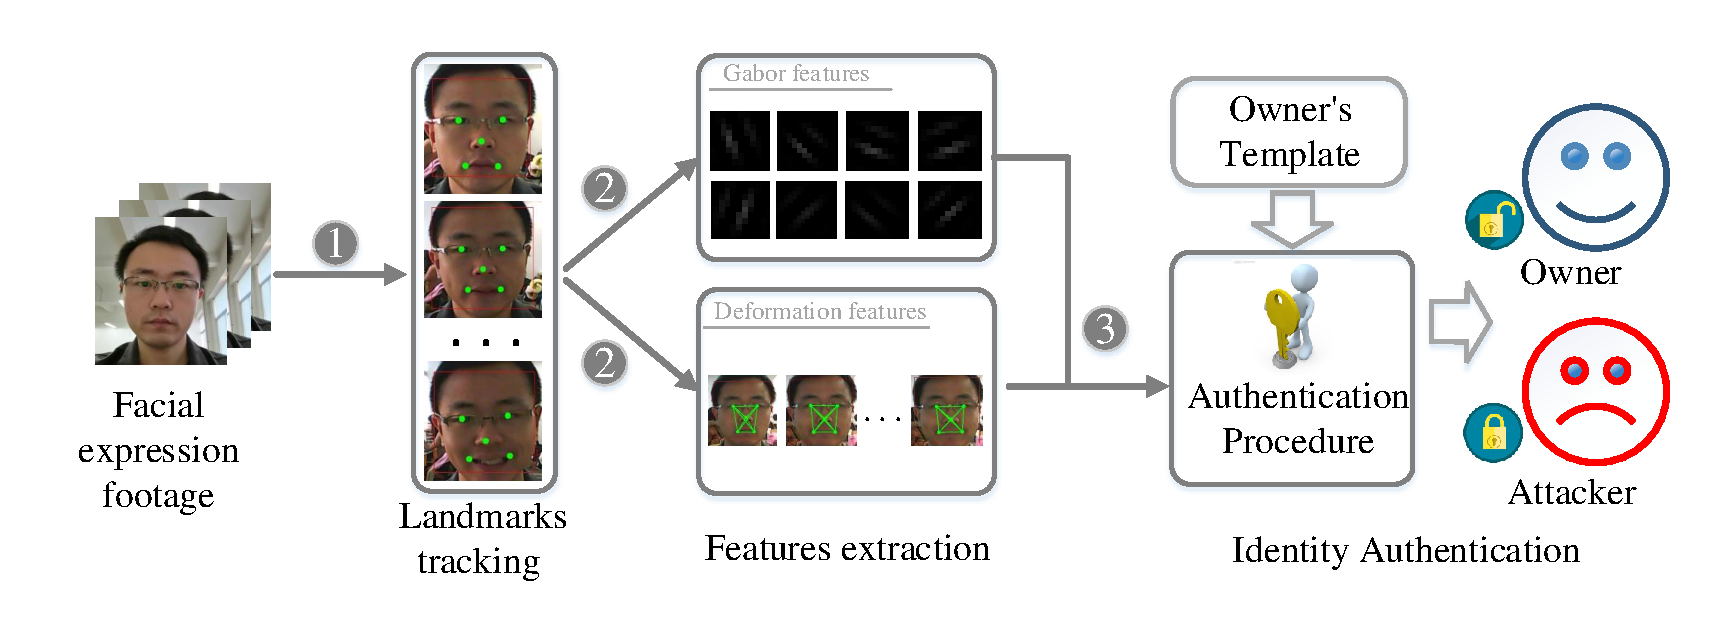
\includegraphics[width=\textwidth]{fig/overview.pdf}
        \caption{Overview of the attack.}
        \label{fig:overview}
    \end{figure*}
    \subsection{Design Goals}
        Biometrics which refers to either the static physiological traits or dynamic behavioral modalities are all non-revocable. This is one of the major reasons why biometrics is possible to be stolen or replayed by an expert adversary. Unlike traditional biometrics, facial behavioral traits is unique and can be changed with the changes of facial expressions. This is the biggest difference comparing with other biometric-based authentication systems. Therefore, facial behavior-based modalities are more secure than other biometrics in some extent.  Furthermore, it is possible to decrease the authentication time as much as possible with the development of facial detection technologies as well as not requiring the visual stimuli. This making facial biometrics are more user-friendly. In conclusion, a secure biometric-based authentication system should be secure, fast and user-friendly. The following we summary the design goals of our system:
        \begin{itemize}
            \item \emph{Simple:} This system should be simple as much as possible. Specifically, user should be minimal coordinate the system during authenticating process.
            \item \emph{Fast:} A single authentication duration should be as short as possible.
            \item \emph{Secure:} The system is able to immune to the replay and impersonation attacks.
            \item \emph{Revocable:} The biometrics can be changed once it is stolen or leakage.
        \end{itemize} 
    
    \subsection{System Overview}
        The system authenticates the user's identity by analyzing the dynamic changes of facial expressions. It records the entire change of facial expressions using in-built front camera of smartphone. The deformation features of facial expressions are extracted by existing facial detection algorithm and they are used to recognize the user's identity.
        Figure ~\ref{fig:overview} depicts the steps of this system:
         
\section{Implementation Details}
    \subsection{Facial Landmarks Tracking and normalizing}
        The first step of this authentication system is to track the facial landmarks from the video footage. We achieve this by employing an open source facial tracking algorithm called SeetaFace~\cite{SeetaFace-toolbox-web}. This algorithm can real-time detect human face and tracks the facial landmarks based on deep convolutional neural network (CNN)~\cite{Krizhevsky2012ImageNet}. For each video frame, the algorithm tries to localize the position of the facial landmarks.
        \subsubsection{Track Facial Landmarks}
            The SeetaFace algorithm automatically detects and tracks face landmarks based on the deep CNN model trained offline. For each video frame, the algorithm first detects the face using scan window mechanism. The size of scan window has an prominent effect on real-time detection speed. We set the window size to no less than $50$ which is found to give good tradeoff between the detection speed and accuracy in our initial design experiment using $35$ expression videos\footnote{To provide a fair evaluation, the video footages used in all our initial test runs in the design phase are different from the ones used later in evaluation}. SeetaFace has three modules: (1) face detection module that follows the face across consecutive frames under the assumption that the frame-to-frame facial expressions are visible; (2) face alignment module that tracks the facial landmarks and localize its position on the face based on the face area detected in (1); and (3) face identification module that is applied to recognize human's identify by simply calculating the cosine similarity of two facial images. It is worthwhile to mention that our system just employs the first two modules which is enough for our system to get the position of facial landmarks.

            The SeetaFace face detection module is constructed by using Funnel-Structured (\emph{FuSt}) cascade scheme. The \emph{FuSt} cascade scheme consists of coarse-to-fine cascade classifiers: multiple view-specific fast LAB  cascade for coarse face selection at the top stage, followed by the coarse Multilayer Perceptron (\emph{MLP}) cascade for facial candidate windows verification at the middle stage and a fine \emph{MLP} cascade for localize the face position at the bottom stage~\cite{Wu2016Funnel}. In the following frames, the detection module detects the face based on a model trained in advance with approximately $200K$ labeled face images by using the above three coarse-to-fine cascade classifiers. For each video frame, the face module detects the potential face areas according to the sliding window paradigm and finally yields the face area by going through the cascade classifiers stage by stage. Taking the detected face area as an input, the face alignment module localize the facial landmarks by exploiting a Coarse-to-Fine Auto-encoder Networks (\emph{CFAN})~\cite{Zhang2014Coarse}. The \emph{CFAN} is comprised of a few successive Stacked Auto-encoder Network (\emph{SANs}). The first \emph{SAN} aims to predicts the approximate facial landmark locations based on the detected face area and then the following \emph{SANs} progressively refine the landmark locations by the joint local features extracted around the current landmarks. Finally, the five facial landmarks locations will be stored for further feature extraction. Detail discussion of SeetaFace can be found at~\cite{SeetaFace-toolbox-web}. Sometimes the algorithm may fail to detect the face in some video frames due to drastically head pose. If this happen, our algorithm will tolerate a certain degree of detection failure but it will ask the user re-authenticate if many detection failure (more than 30\%) occurs.

        \begin{figure}
            \centering
            \subfigure{
                \begin{minipage}[t]{0.19\textwidth}
                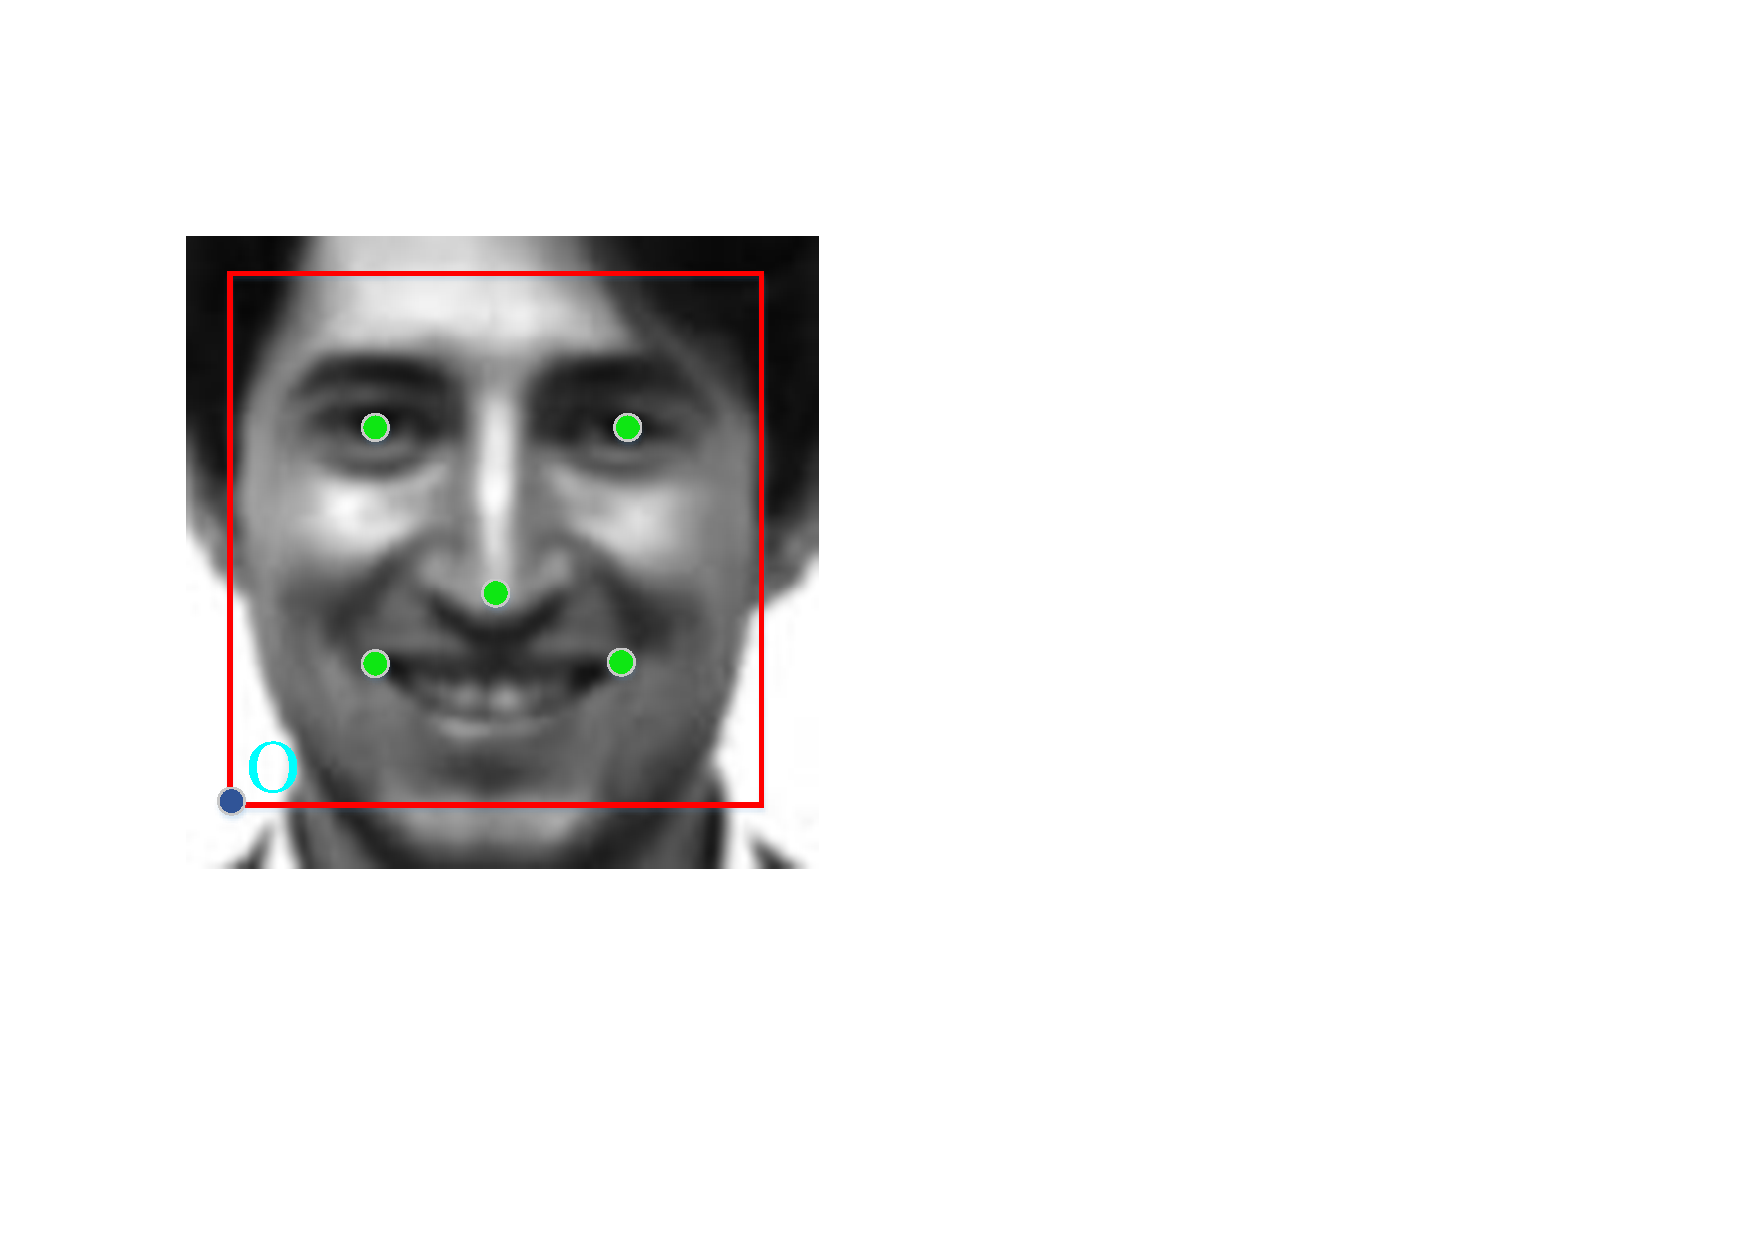
\includegraphics[width=0.8\textwidth]{fig/normalization1.pdf}\\
                \centering \footnotesize (a) a frontal-view face
                %\FIXME{Need to mark the starting point and turning point}
                \end{minipage}
            }
            \hspace{0.25cm}
            \subfigure{
                \begin{minipage}[t]{0.19\textwidth}
                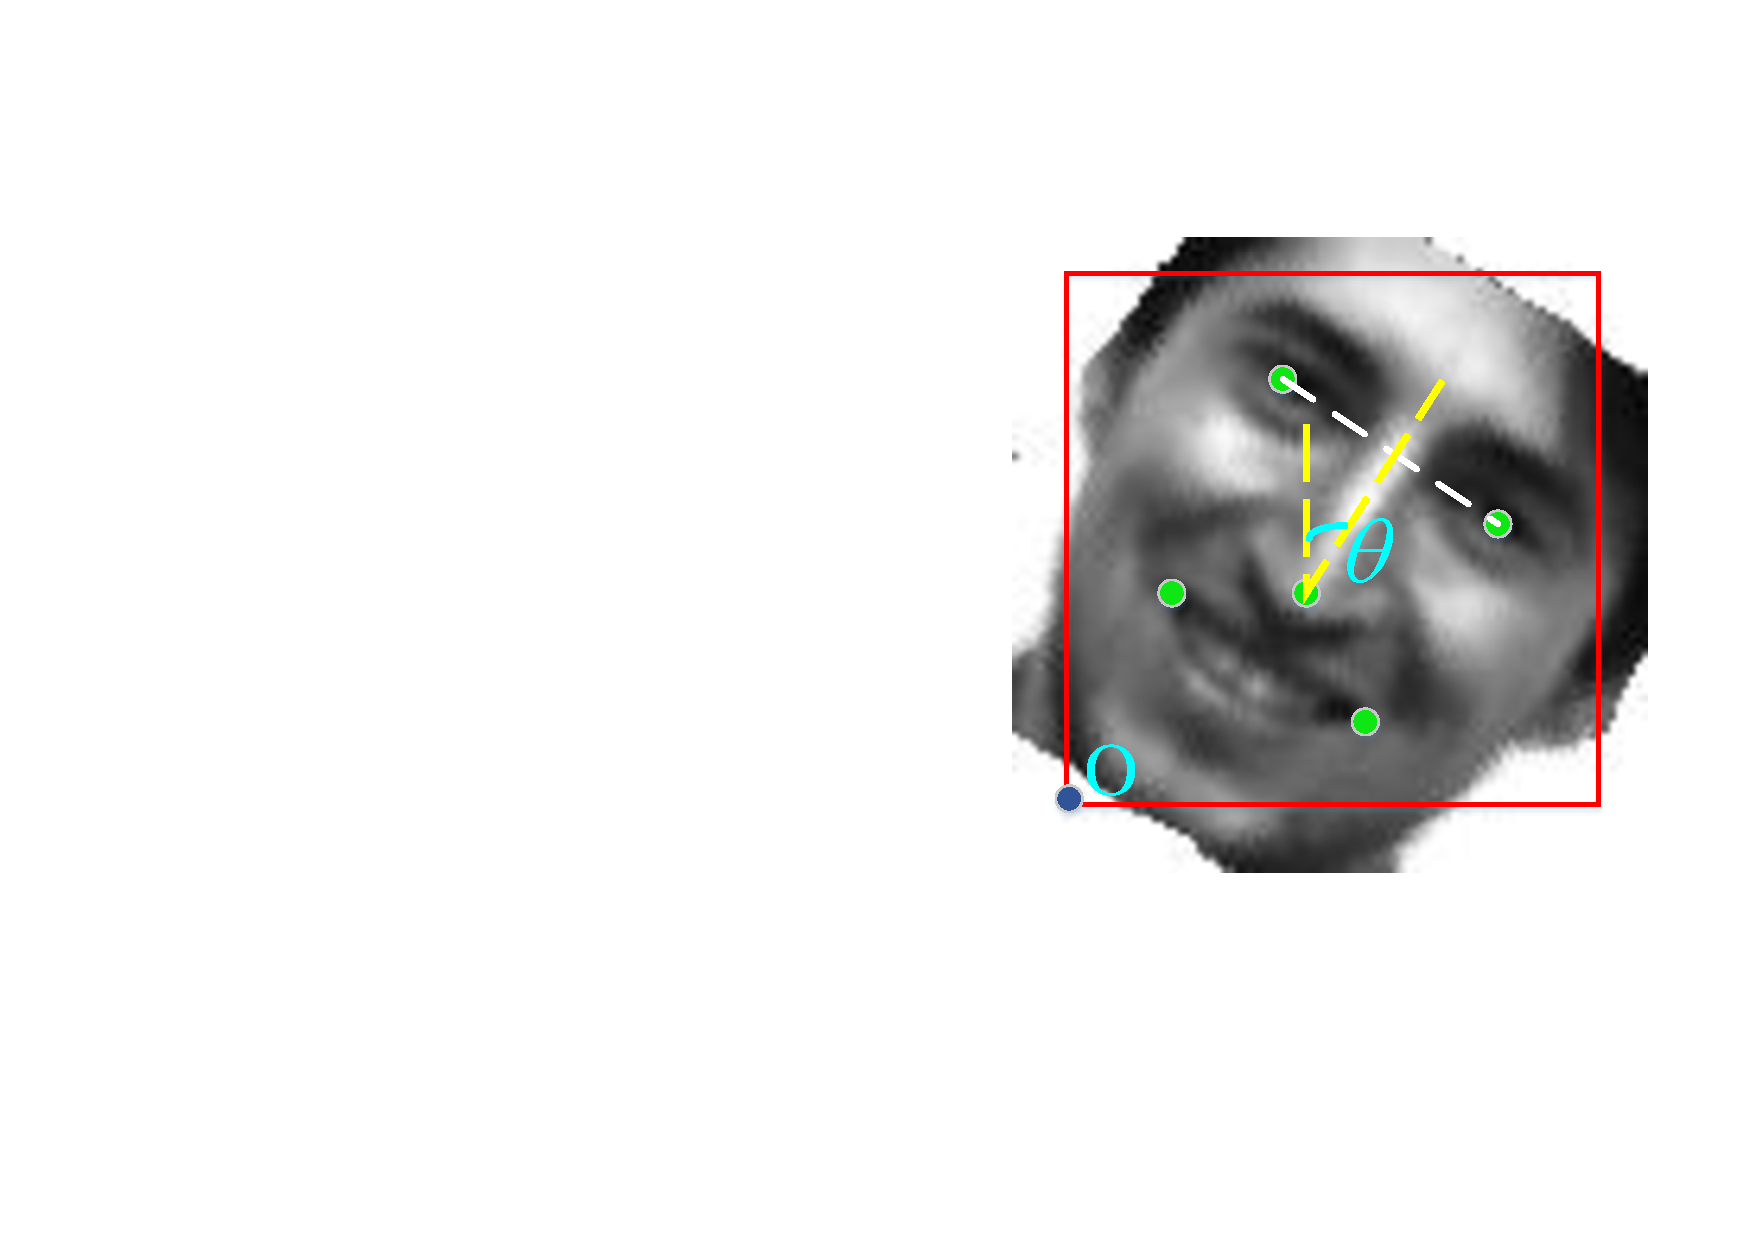
\includegraphics[width=0.8\textwidth]{fig/normalization2.pdf}\\
                \centering \footnotesize (b) a camera's view face
                \end{minipage}
            }
            \caption{Facial expressions and landmarks under two different view angles. The rotation angle, $\theta$, is the angle between the midperpendicular of connection of two eye landmarks and a vertical line.}
            \label{fig:normalization}
        \end{figure}
        
        \begin{algorithm}[!t]
            \centering
            \caption{Face Normalization Algorithm}
            \small
            \label{alg:normalization}
            \begin{algorithmic}[1]
                \REQUIRE~~\\
                    $EV$: Expression Video  \\
                    $angleThreshold$: The threshold of rotation angle\\
                    $fixedSize$: The fixed size of uniform facial images\\
                    %$locationTh$: Threshold of fingertip location changes\\
                \ENSURE~~\\
                    %$<$start,end$>$: Start and end of the unlocking video segment \\
                    $NF[]$: Normalized facial expression images under frontal view\\
                \STATE $flag \leftarrow openFrontFacingCamera()$
                \WHILE{$flag$}
                    \STATE $eF \leftarrow captureExpressionFrames()$ \\
                    \IF{$!ef$}
                        \STATE $fL[] \leftarrow getFacialLandmarks(eF)$ \\
                        \STATE $rA \leftarrow calculateRotationAngle(fL[])$
                        \IF{$rA>angleThreshold$}
                            \STATE $fI \leftarrow rotateFacialFrame(eF,rA)$
                        \ELSE
                            \STATE $fI \leftarrow eF$
                        \ENDIF
                        \STATE $NF[] \leftarrow zoomFacialImage(fI,fixedSize)$
                    \ENDIF
                \ENDWHILE
            \end{algorithmic}
        \end{algorithm}
        \subsubsection{Face Normalization}
            By default, The face alignment algorithm reports the facial landmarks positions with respect to the bottom-left pixel of the face shown as Figure~\ref{fig:normalization} (a) point $O$. However, the size of face detected by face detection module are uniform under different usage scenarios as the distance between the face and the phone camera are not the same according to individual's habits. For example, this distance when one lies in bed is typically shorter than the one when he stands or sits. Furthermore, the head pose still results in the rotation of the face in specific situation such as playing the smartphone in bed. Those can drastically affect the value of the dynamic facial features, leading to misidentification of users in authentication phase.

            Our approach to solve the above challenges can be divided into two steps. The first step is to rotate the face from the camera's view to the frontal view. To do so, we need to evaluate the rotation angle of the face. If the value of rotation angle is more than a threshold, this approach will automatically rotate the face to the frontal side. The rotation angle can be figured out according to the part of the facial landmarks including the left and right center of the eyes and the nose tip. This is illustrated in Figure~\ref{fig:normalization} (b). Based on the estimated filming angle, $\theta$, we use the following formula to transform the face from the camera's view to the frontal view:
            \begin{equation}
                P=TP^{'} \qquad, \qquad  T=\left[ \begin{matrix} \cos\theta & -\sin\theta \\ \sin\theta & \cos\theta \end{matrix} \right]
            \end{equation}

            where $T$ is a Transformation Matrix, $P^{'}$ is the coordinate of a point of the face, and $P$ is the resulting coordinate after the transformation. For each video frame, our algorithm individually calculates the rotate angle and perform the transformation, because the rotation angle may change across video frames.

            The second step is to normalize the facial size. To uniform the face size, we map the face detected by face detection module to a fixed size which is $200\times200$ pixels. To do so, our algorithm uses the bilinear interpolation algorithm~\cite{Gribbon2004A} to zoom in/out the current face comparing to the fixed size.

            The algorithm for face normalization process is described in Algorithm~\ref{alg:normalization}. The input to the algorithm is the facial expression video footage and the threshold of rotation angle, and the output of the algorithm is the frontal facial images. To normalize the facial expression images, we first figure out the rotation angle. To do so, the coordinates of the five facial landmarks are tracked (line 5), and the rotation angle can be calculated according to the angle between the vertical ling and the midperpendicular of connection line of two eyes landmarks (line 6). IF the rotation angle is more than a threshold, $angleThreshold$, the facial expression image will be rotated to frontal view and zoomed in/out to the fixed size (lines 8 and 12).  Specifically, the angle threshold, $angleThreshold$, is set to 5 and the fixed size of facial images, $fixedSize$ is set to $200\times200$ pixels. To determine the thresholds, we have evaluated a range of possible values in our initial design experiments to chose the best performing values.

    \subsection{Replay Detection}
        
    \subsection{Feature Extraction}

    \subsection{Identity Authentication}


%1. Smartphone is easily lost or stolen by an attacker as its small size. This may result in privacy leakage and finance lost. It is reported by lookout.com that nearly \$2.5 billion worth of devices were lost or stolen in 2011~\cite{lookout-survey}.

2. Human face plays an important role in our social interaction. As compared with other biometric modalities such as fingerprint and iris, face recognition has distinct advantages because of its non-contact process. Face images could be captured from a distance without touching person being identified and identification does not require interaction with person. In addition, face recognition serves crime deterrent purpose because face images that have been recorded and archived could later help identify a person.

3. Human identification system based on biometrics other than the face have already led to commercial products with very high identification rates: the iris~\cite{daugman1993high} and fingerprints~\cite{rogers1994biometric} can be cited as example. However, these systems are not always appreciated by users, as they require some close interaction with the machine often perceived as invasive. Moreover, they require the user to stop at the device and be cooperative, which is acceptable for access control to restricted areas, but not for other applications like surveillance. Face recognition may overcome some of these limitations.

4. Challenges in face recognition arise because the face is not a rigid object and images can be taken from many different viewpoints of the face.

5. Biometric-based techniques have emerged as the most promising option for recognizing individuals in recent years since, instead of authenticating people and granting them access to physical and virtual domains based on passwords, PINs, smart cards, plastic cards, tokens, keys and so forth, thses methods examine an individual's physiological and/or behavioral characteristics in order yo determine and/or ascertain his identity. Passwords and PINs are hard to remember and can be stolen or guessed; cards, tokens, keys and the like can be misplaced, forgotten, purloined or duplicated; magnetic cards can become corrupted and unreadable. However, an individual's biological traits cannot be misplaced, forgotten, stolen or forged.

Biometric-based technologies include identification based on physiological characteristics (such as face, fingerprints, finger geometry, hand geometry, hand veins, palm, iris, retina, ear and voice) and behavioral traits (such as gait, signature and keystroke dynamics). Face recognition appears to offer several advantages over other biometric methods as follows:

\begin{itemize}
    \item Almost all these technologies require some voluntary action by the user, i.e., the user needs to place his hand on a hand-rest for fingerprinting or hand geometry detection and has to stand in a fixed position in front of a camera for iris or retina identification. However, face recognition can be done passively without any explicit action or participation on the part of the user since face images can be acquired from a distance by a camera. This is particulary beneficial for security and surveillance purposes.
    \item Data acquisition in general is fraught with problems for other biometrics: techniques that rely on hands and fingers can be rendered useless if the epidermis tissue is damaged in some way (i.e., bruise or cracked). Iris and retina identification require expensive equipment and are much too sensitive to any body motion. Voice recognition is susceptible to background noises in public places and auditory fluctuations on a phone line or tape recording. Signatures can be modified or forged. However, facial images can be easily obtained with a couple of inexpensive fixed cameras.
    \item Good face recognition algorithms and appropriate preprocessing of the images can compensate for noise and slight variations in orientation, scale and illumination.
    \item Technologies that require multiple individuals to use the same equipment to capture their biological characteristics potentially expose the user to the transmission of germs and impurities from other users. However, face recognition is totally non-intrusive and does not carry any such health risks.
\end{itemize}

6. In this section, we discuss the technical considerations that underpin the design of CarSafe while the detailed design is presented in section 3.  CarSafe fundamentally relies on the real-time processing of dual camera video streams. In what follows, we discuss the challenges and design considerations that arise.  This example motivates the need for the simultaneously processing of video streams from the front and rear cameras. SURF features are provided to a binary two-class SVM that is trained to classify eyes as either being open or closed (defined as an open or closed event).

7. Related Work--Face recognition techniques can be broadly divided into three categories based on the face data acquisition methodology: methods that operate on intensity images; those that deal with video sequences; and those that require other sensory data such 3D information or infra-red imagery~\cite{Jafri2009A}.

8. Among our interesting finding is how large a role web passwords play in user lives. The average user has 6.5 passwords, each of which is shared across 3.9 different sites. Each user has about 25 accounts that require passwords, and types an average of 8 passwords per day~\cite{florencio2007}.

9. With the advances in miniaturization techniques, performance of the mobile and portable devices is rapidly increasing. This enables to use such devices not only as communication tools but also in an applications like m-banking~\cite{Pousttchi2004Assessment} or m-government~\cite{Kim1970Architecture}. This means that they can store and process valuable information such as financial or private data. According to UK statistics in every three minutes a mobile phone is stolen~\cite{hugeSurge2006}. The current protection mechanisms of these devices are usually based on PIN code or passwords. Nowadays a "heavy" user has on average 21 passwords to remember~\cite{2002NATMonitor}. Unfortunately, 81\% of the users select common words as a passwords and 30\% of users write their passwords down, which equally compromises security~\cite{2002NATMonitor}. Recently, biometric modalities such as fingerprints~\cite{Su2005A,Chen2005A} have been proposed for mobile devices. However, both fingerprints and password entry are obtrusive and require explicit action from the user, which is not convenient in a frequent use. In order to improve security in mobile and portable devices, an unobtrusive mechanisms of authentication is desirable.

10. Geometric Deformation Features. The geometric displacement of certain selected Candide node,defined as the difference of the node coordinates between the first and the greatest facial expression intensity frame, is used as an input to a novel multiclass Support Vectot Machine (SVM) system of classifiers that are used to recognize either the six basic facial expressions or a set of chosen Facial Action Units (FAUs).
\textbf{The leave-one cross-validation approach was used in order to make maximal use of the available data and produce averaged classification accuracy results.}~\cite{Kotsia2007Facial}.

11. The benefits of feature selection are not only to reduce recognition time by reducing the amount of data that needs to be analyzed, but also, in many cases, to produce better classification accuracy due to finite sample size effects~\cite{Jain1997Feature}.

%\section{Related Work}
    Our work lies at the intersection between human face recognition and biometric-based authentication methods. We bring together techniques developed in the domain of face recognition and identity authentication to develop a new authentication scheme.

    \noindent \textbf{Physiological biometrics}

    \noindent \textbf{Behavioral biometrics}

    \noindent \textbf{Face recognition} The approaches reported regarding facial expression recognition can be distinguished in two main directions, the feature-based ones and the template-based ones, according to the method they use for facial information extraction. The feature-based methods use texture or geometrical information as features for expression information extraction. The template-based methods use 3-D or 2-D head and facial models as templates for expression information extraction.
    \begin{itemize}
        \item \textbf{Feature-Based Approaches:} Facial feature detection and tracking is based on active InfraRed illumination in~\cite{Zhang2005Active}, in order to provide visual information under variable lighting and head motion. The classification is performed using a Dynamic Bayesian Network (DBN).
            A method for static and dynamic segmentation and classification of facial expression is processed in~\cite{Cohen2003Facial}. For the static case, a DBN id used, organized in a tree structure. For the dynamic approach, multi level Hidden Markov Models (HMMs) classifiers are employed.
            The system proposed in~\cite{Bartlett2003Real} automatically detects frontal faces in the video stream and classifies them in seven classes in real time: neutral, anger, disgust, fear, joy, sadness, and surprise. An expression recognizer receives image regions produced by a face detector and then a Gabor representation of the facial image region is formed to be later processed by a bank of SVMs classifiers.
            Gabor filters are also used in~\cite{Lyons1998Coding} for facial expression recognition. Facial expression images are coded using a multiorientation, multiresolution set of Gabor filters which are topographically ordered and aligned approximately with the face.
            A Neural Network (NN) is employed to performe facial expression recognition in~\cite{Zhang1998Comparison}. The features used can be either the geometric positions of a set of fiducial points on a face or a set of multiscale and multiorientation Gabor eavelet coefficients extracted from the facial image at the fiducial points.
            A convolutional NN was used in~\cite{Fasel2002Multiscale}. The system developed is robust to face location changes and scale variations. Feature extraction and facial expression classification were performed using neuron groups, having as input a feature map and properly adjusting the weights of the neurons for correct classification.

        \item \textbf{Model Template-Based Approaches:} A 3-D facial model used for facial expression recognition is also proposed in~\cite{Braathen2002An}. First, the head pose is estimated in a facial video sequences. Subsequently, face images are wraped onto a face model with canonical face geometry, then they are rotated to frontal ones, and are projected back onto the image plane. Pixels brightness is linearly rescaled and resulting images are convolved with a bank of Gabor kernels. The Gabor representations are then channelled to a bank of SVMs to perform facial expression recognition.
    \end{itemize}


    \noindent \textbf{Expression recognition}


\section*{Acknowledgements}
    We would like to thank all participants who help for completing the experiments. Thank all volunteers for their time and insights as well as the anonymous reviewer for their critical and constructive comments. This work was supported by NSFC (Grant No. 61672427) and the UK Engineering and Physical Sciences Research Council (Grants No. EP/M01567X/1(SANDeRs) and EP/M015793/1(DIVIDEND)).

%\begin{spacing}{0.98}
\bibliographystyle{IEEEtranS}
\balance
\bibliography{refs}
%\end{spacing}

\end{document}
